
\cxset{style70/.style={
 name={Chapter},
 chapter color = ,
 chapter toc = true,
 numbering=arabic,
 number font-size=Large,
 number font-family=rmfamily,
 number font-weight=\normalfont\itshape,
 number color= black,
 number before=\kern0.5em,
 number dot=,
 number after=\hfill,
 number position= rightname,
 chapter font-family=rmfamily,
 chapter font-weight= \itshape,
 chapter font-size=\Large,
 chapter before={\hrule height2pt width \columnwidth\kern3.5pt% 
\hrule height2pt width \columnwidth \kern3.5pt%
\hrule height2pt width \columnwidth 
\kern12.6pt \par\hfill},
 chapter after=,
 chapter color=black!90,
 chapter spaceout=none,
%title beforeskip={\vspace*{10pt}},
% title afterskip={\vspace*{30pt}\par},
 title margin top=10pt,
 title margin bottom=10pt,
 title before=,
 title after=,
 title font-family=rmfamily,
 title font-color=black!90,
 title font-weight=bfseries,
 title font-size=huge,
 title spaceout=none,
 chapter title align=centering,
 title font-shape = normal,
 header style= headings,
 author block=true}}

\cxset{style70}
\chapter{Introduction to Style Five}\index{styles!style5}

\tcbset{width=\textwidth}
I think this style can be improved with a bit of color. You can experiment with it quite easily. The spacing on top of this style can also be adjusted to suit your typographical taste.
\medskip
\begin{figure}[ht]
\centering
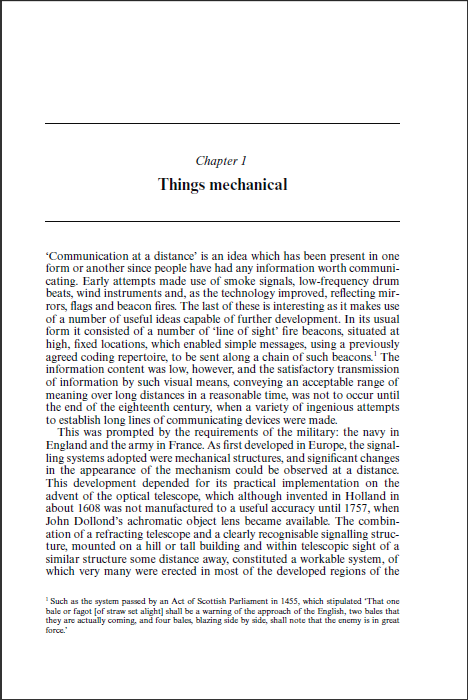
\includegraphics[width=0.6\textwidth]{./chapters/chapter05.png}
\end{figure}

%\section{General notes on rules}

LaTeX's default rules would normally give problems. Best is to use TeX's primitives to built them.




\section{Images}

\begin{figure}[htbp]
\centering
\includegraphics[width=0.8\textwidth]{telegraphy}
\caption{Spread from the \textit{History of Telegraphy}, the caption is set left and the image is centered.}
\end{figure}
